\documentclass[10pt, aspectratio=169]{beamer}

% --- Cấu hình Tiếng Việt & Theme ---
\usepackage{fontspec}
\usetheme[progressbar=frametitle]{metropolis}
\usepackage{appendixnumberbeamer}

% --- Thư viện cần thiết ---
\usepackage{booktabs}
\usepackage[scale=2]{ccicons}
\usepackage{pgfplots}
\usepgfplotslibrary{dateplot}
\usepackage{amsmath, amssymb}
\usepackage{bm} 
\usepackage{tikz} 
\usetikzlibrary{shapes, arrows, positioning}

% --- Cấu hình Đường dẫn & Màu sắc ---
\graphicspath{{img/}} % Chỉ định thư mục chứa ảnh
\definecolor{DarkBlue}{HTML}{003366}
\setbeamercolor{palette primary}{bg=DarkBlue}

% --- Metadata ---
\title{From Geometric Intuition to Real‑world Deployment with Support Vector Machines}
% \subtitle{Tối ưu hóa hình học trong kỹ nghệ AI}
\date{\today}
\author{Long Nguyen Hoang}
\institute{University of Information Technology - VNU-HCM \\ Faculty of Information Science and Engineering}
\titlegraphic{\hfill
\includegraphics[height=1cm]{logo_uit.png}}

\begin{document}

\maketitle

\begin{frame}{Nội dung bài chia sẻ}
  \setbeamertemplate{section in toc}[sections numbered]
  \tableofcontents[hideallsubsections]
\end{frame}

% --- Import các Chương ---
\section{The Linear Intuition}

% ====================================================
% --- Slide 1: Thiết lập trực giác (Không có toán) ---
% ====================================================
\begin{frame}{Bài toán phân loại trên mặt phẳng}
  \begin{columns}
    \begin{column}{0.4\textwidth}
      \begin{itemize}
        \item Cho hai nhóm dữ liệu: \textcolor{blue}{Nhóm A} và \textcolor{red}{Nhóm O}.
        \item Mục tiêu: Tìm một \textbf{đường ranh giới} để phân tách chúng.
        \item Có \textbf{vô số} cách vẽ đường thẳng.
        \item \textit{Vậy đâu là ranh giới hợp lý nhất?}
      \end{itemize}
    \end{column}
    
    \begin{column}{0.6\textwidth}
      \centering
      \begin{tikzpicture}[scale=1.2]
        % Vẽ khung trục tọa độ nhẹ nhàng
        \draw[->, gray!50] (-0.5,0) -- (5,0) node[right] {$x_1$};
        \draw[->, gray!50] (0,-0.5) -- (0,4) node[above] {$x_2$};

        % Nhóm A (màu xanh)
        \filldraw[blue] (3,3) circle (2pt);
        \filldraw[blue] (4,2.5) circle (2pt);
        \filldraw[blue] (2.5,4) circle (2pt);
        \filldraw[blue] (4,3.5) circle (2pt);
        \filldraw[blue] (3.2,2.8) circle (2pt);

        % Nhóm O (màu đỏ)
        \filldraw[red] (1,0.5) rectangle (1.2,0.7);
        \filldraw[red] (2,-0.2) rectangle (2.2,0);
        \filldraw[red] (0.5,1) rectangle (0.7,1.2);
        \filldraw[red] (1.8,0.8) rectangle (2.0,1.0);
        \filldraw[red] (0.8,1.8) rectangle (1.0,2.0);
      \end{tikzpicture}
    \end{column}
  \end{columns}
\end{frame}

% ====================================================
% --- Slide 2: Khớp nối trực giác vào Công thức ---
% ====================================================
\begin{frame}{Ý tưởng cốt lõi: Đường ranh giới an toàn nhất}
  \begin{columns}
    \begin{column}{0.4\textwidth}
      \textbf{Làm sao để chọn đường tốt nhất?}
      \vspace{0.3cm}
      \begin{enumerate}
        \item Hãy tưởng tượng một \textbf{"con đường"} càng rộng càng tốt để phân tách hai nhóm.
        \item \textbf{Đường ranh giới} sẽ nằm chính giữa con đường đó.
        \item Những điểm nằm sát mép đường được gọi là \textbf{Support Vectors} (Điểm trụ cột).
      \end{enumerate}
      \vspace{0.3cm}
      \textbf{Kết luận:} Đường thẳng \textit{an toàn nhất} là đường có \textbf{lề đường rộng nhất}.
    \end{column}
    
    \begin{column}{0.6\textwidth}
      \centering
      \begin{tikzpicture}[scale=1.2, >=stealth]
        % Trục tọa độ
        \draw[->, gray!50] (-0.5,0) -- (5,0);
        \draw[->, gray!50] (0,-0.5) -- (0,4);

        % Dữ liệu lớp Xanh
        \filldraw[blue] (3,3) circle (2pt);
        \filldraw[blue] (4,2.5) circle (2pt);
        \filldraw[blue] (2.5,4) circle (2pt);
        \filldraw[blue] (4,3.5) circle (2pt);
        \filldraw[blue] (3.2,2.8) circle (2pt);
        
        % Support Vector Xanh (nằm sát mép)
        \filldraw[blue] (2,3.5) circle (2.5pt);
        \draw[blue, thick] (2,3.5) circle (5pt);
        \node[blue] at (1.5, 3.8) {SV};

        % Dữ liệu lớp Đỏ
        \filldraw[red] (1,0.5) rectangle (1.2,0.7);
        \filldraw[red] (2,-0.2) rectangle (2.2,0);
        \filldraw[red] (0.5,1) rectangle (0.7,1.2);
        \filldraw[red] (1.8,0.8) rectangle (2.0,1.0);
        
        % Support Vector Đỏ (nằm sát mép)
        \filldraw[red] (1.4,1.4) rectangle (1.6,1.6);
        \draw[red, thick] (1.5,1.5) circle (5pt);
        \node[red] at (1.0, 1.0) {SV};

        % Đường ranh giới chính giữa
        \draw[ultra thick, DarkBlue] (0.2, 3.3) -- (3.8, -0.3) node[below right] {\footnotesize Ranh giới};

        % Đường biên (Margin)
        \draw[dashed, thick, DarkBlue!60] (0, 2.5) -- (3, -0.5);
        \draw[dashed, thick, DarkBlue!60] (1, 4.5) -- (4.5, 1.0);

        % Mũi tên chỉ khoảng cách Margin
        \draw[<->, black, thick] (1.3, 2.2) -- (2.3, 3.2) node[midway, sloped, above] {\small Margin};
      \end{tikzpicture}
    \end{column}
  \end{columns}
\end{frame}

% ================================================
% SLIDE 3
% ================================================
\begin{frame}{Biểu diễn ranh giới trong không gian 2 chiều}
  \begin{columns}
    \begin{column}{0.45\textwidth}
      Một đường thẳng trên mặt phẳng $\mathbb{R}^2$ có dạng:
      \[
      w_1 x_1 + w_2 x_2 + b = 0
      \]
      \vspace{0.2cm}
      \textbf{Ý nghĩa các thành phần:}
      \begin{itemize}
        \item $\vec{w} = (w_1, w_2)$: vector \textbf{vuông góc} với đường thẳng, quyết định \textit{hướng}.
        \item $b$: điều chỉnh \textit{vị trí} (tịnh tiến song song).
      \end{itemize}
      \vspace{0.3cm}
      Khi thay tọa độ điểm $A(x_1^A, x_2^A)$ vào vế trái, dấu của kết quả cho biết điểm nằm \textit{phía nào} của đường thẳng.
    \end{column}
    \begin{column}{0.55\textwidth}
      \centering
      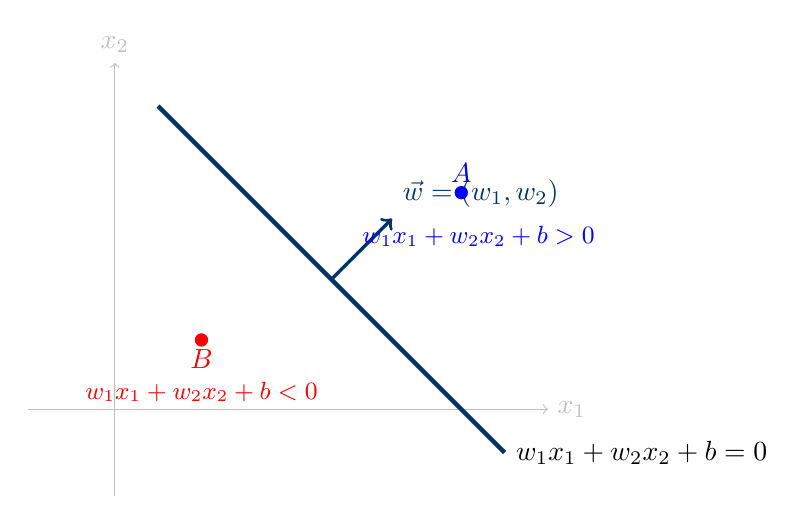
\begin{tikzpicture}[scale=1.1]
        \draw[->, gray!50] (-1,0) -- (5,0) node[right] {$x_1$};
        \draw[->, gray!50] (0,-1) -- (0,4) node[above] {$x_2$};
        % Đường thẳng
        \draw[ultra thick, DarkBlue] (0.5,3.5) -- (4.5,-0.5) node[right, text=black] {$w_1 x_1 + w_2 x_2 + b = 0$};
        % Vector pháp tuyến
        \draw[->, very thick, DarkBlue] (2.5,1.5) -- (3.2,2.2) node[above right] {$\vec{w} = (w_1, w_2)$};
        % Điểm minh họa
        \filldraw[blue] (4,2.5) circle (2pt) node[above] {$A$};
        \filldraw[red] (1,0.8) circle (2pt) node[below] {$B$};
        % Ghi chú dấu
        \node[blue] at (4.2,2) {\small $w_1 x_1 + w_2 x_2 + b > 0$};
        \node[red] at (1,0.2) {\small $w_1 x_1 + w_2 x_2 + b < 0$};
      \end{tikzpicture}
    \end{column}
  \end{columns}
\end{frame}

% ========================================================
% Slide 4: Toán học tổng quát
% ========================================================
\begin{frame}{Tổng quát hóa: Siêu phẳng và bài toán}
  \begin{block}{Từ 2D đến không gian $d$ chiều}
    Trong không gian nhiều chiều, ranh giới là một \textbf{siêu phẳng}:
    \[
    \bm{w}^T \bm{x} + b = 0
    \]
    với $\bm{w} \in \mathbb{R}^d$, $b \in \mathbb{R}$.
  \end{block}

  \begin{columns}
    \begin{column}{0.5\textwidth}
      \textbf{Khoảng cách từ điểm đến siêu phẳng:}
      \[
      d = \frac{|\bm{w}^T \bm{x} + b|}{\|\bm{w}\|}
      \]
      \vspace{0.2cm}
      \textbf{Mục tiêu phân loại:}
      \begin{itemize}
        \item Điểm lớp xanh (+1): $\bm{w}^T \bm{x} + b \geq +1$
        \item Điểm lớp đỏ (-1): $\bm{w}^T \bm{x} + b \leq -1$
      \end{itemize}
      $\Rightarrow y_i (\bm{w}^T \bm{x}_i + b) \geq 1, \forall i$
    \end{column}
    \begin{column}{0.5\textwidth}
      \centering
      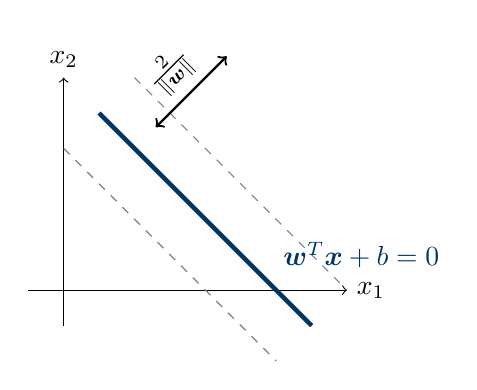
\begin{tikzpicture}[scale=0.9]
        \draw[->] (-0.5,0) -- (4,0) node[right] {$x_1$};
        \draw[->] (0,-0.5) -- (0,3) node[above] {$x_2$};
        \draw[ultra thick, DarkBlue] (0.5,2.5) -- (3.5,-0.5);
        \draw[dashed, DarkBlue!60] (0,2) -- (3,-1);
        \draw[dashed, DarkBlue!60] (1,3) -- (4,0);
        \draw[<->, thick] (1.3,2.3) -- (2.3,3.3) node[midway, above, sloped] {$\frac{2}{\|\bm{w}\|}$};
        \node[DarkBlue] at (4.2,0.5) {$\bm{w}^T\bm{x}+b=0$};
      \end{tikzpicture}
    \end{column}
  \end{columns}
\end{frame}

% ================================================
% Phát biểu mô hình
% ================================================
\begin{frame}{Tổng quát mô hình}
  \textbf{Giả định của mô hình:}
  \begin{itemize}
    \item Dữ liệu huấn luyện $\{(\bm{x}_i, y_i)\}_{i=1}^n$ với $\bm{x}_i \in \mathbb{R}^d$, nhãn $y_i \in \{-1, +1\}$.
    \item \textbf{Tuyến tính khả tách}: Tồn tại ít nhất một siêu phẳng phân tách hoàn toàn hai lớp.
  \end{itemize}

  \vspace{0.3cm}
  \textbf{Mô hình SVM (dạng hard-margin):}
  \begin{block}{Siêu phẳng phân loại}
    \[
    f(\bm{x}) = \bm{w}^T \bm{x} + b
    \]
    \begin{itemize}
      \item Nếu $f(\bm{x}) \ge 0$: dự đoán lớp $+1$ (xanh)
      \item Nếu $f(\bm{x}) < 0$: dự đoán lớp $-1$ (đỏ)
    \end{itemize}
  \end{block}
\end{frame}

\begin{frame}{Tổng quát mô hình}
  \begin{alertblock}{Điều kiện phân loại đúng với margin}
    Để đảm bảo mọi điểm nằm \textbf{ngoài hoặc trên mép lề}, ta yêu cầu:
    \[
    y_i \cdot (\bm{w}^T \bm{x}_i + b) \geq 1, \quad \forall i = 1,\dots,n
    \]
  \end{alertblock}
\end{frame}

% ==============================================
% Điều kiện sử dụng
% ==============================================
\begin{frame}{Điều kiện sử dụng của SVM với biên cứng}
  \begin{columns}
    \begin{column}{0.4\textwidth}
      \textbf{Giả định lý tưởng:}
      \begin{itemize}
        \item Hai lớp \textbf{hoàn toàn tách biệt}.
        \item Không có điểm nhiễu (outlier).
        \item Không có điểm bị gán nhãn sai.
      \end{itemize}
      \vspace{0.3cm}
      Khi đó, tồn tại siêu phẳng phân tách với margin cực đại một cách \textbf{hoàn hảo}.
    \end{column}
    \begin{column}{0.6\textwidth}
      \centering
      \begin{tikzpicture}[scale=1.1]
        \draw[->, gray!50] (-1,0) -- (5,0) node[right] {$x_1$};
        \draw[->, gray!50] (0,-1) -- (0,4) node[above] {$x_2$};
        % Dữ liệu sạch
        \filldraw[blue] (3,3) circle (2pt); \filldraw[blue] (4,2.5) circle (2pt);
        \filldraw[blue] (2.5,4) circle (2pt); \filldraw[blue] (4,3.5) circle (2pt);
        \filldraw[red] (1,0.5) rectangle (1.2,0.7); \filldraw[red] (2,-0.2) rectangle (2.2,0);
        \filldraw[red] (0.5,1) rectangle (0.7,1.2); \filldraw[red] (1.8,0.8) rectangle (2.0,1.0);
        % Siêu phẳng
        \draw[ultra thick, DarkBlue] (0.2,3.3) -- (3.8,-0.3);
        \draw[dashed, DarkBlue!60] (0,2.5) -- (3,-0.5);
        \draw[dashed, DarkBlue!60] (1,4.5) -- (4.5,1);
        \draw[<->, thick] (1.3,2.2) -- (2.3,3.2) node[midway, above, sloped] {Margin rộng};
      \end{tikzpicture}
    \end{column}
  \end{columns}
\end{frame}

\begin{frame}{Điểm yếu của các mô hình Linear SVM}
  \begin{columns}
    \begin{column}{0.4\textwidth}
      Trong thực tế:
      \begin{itemize}
        \item Dữ liệu thường bị \textbf{chồng lấn nhẹ}.
        \item Xuất hiện \textbf{outlier} (điểm nằm sai vùng).
        \item Có thể có \textbf{nhãn bị sai}.
      \end{itemize}
      \vspace{0.3cm}
      \textbf{Hậu quả:} Không thể vẽ được một siêu phẳng vừa phân tách đúng \textit{tất cả} điểm, vừa có margin hợp lý.
    \end{column}
    \begin{column}{0.6\textwidth}
      \centering
      \begin{tikzpicture}[scale=1.1]
        \draw[->, gray!50] (-1,0) -- (5,0) node[right] {$x_1$};
        \draw[->, gray!50] (0,-1) -- (0,4) node[above] {$x_2$};
        % Dữ liệu
        \filldraw[blue] (3,3) circle (2pt); \filldraw[blue] (4,2.5) circle (2pt);
        \filldraw[blue] (2.5,4) circle (2pt); \filldraw[blue] (4,3.5) circle (2pt);
        \filldraw[red] (1,0.5) rectangle (1.2,0.7); \filldraw[red] (2,-0.2) rectangle (2.2,0);
        \filldraw[red] (0.5,1) rectangle (0.7,1.2); \filldraw[red] (1.8,0.8) rectangle (2.0,1.0);
        % Điểm nhiễu (outlier) - màu xanh nằm lẫn vùng đỏ
        \filldraw[blue] (0.8,2.5) circle (2.5pt);
        \draw[->, red, thick] (0.8,2.5) -- (2.5,2) node[midway, above] {Outlier!};
        % Hard-Margin cố gắng vẽ siêu phẳng
        \draw[ultra thick, DarkBlue, opacity=0.4] (1.5,4) -- (4.5,-1);
        \draw[dashed, DarkBlue!60, opacity=0.4] (1,3.5) -- (3.5,-0.5);
        \draw[dashed, DarkBlue!60, opacity=0.4] (2,4.5) -- (5.5,-0.5);
        \node[DarkBlue] at (4.5,0) {\small Margin bị ép hẹp};
      \end{tikzpicture}
    \end{column}
  \end{columns}
\end{frame}

\begin{frame}{Điểm yếu của các mô hình Linear SVM}
  \begin{block}{Ràng buộc cứng}
    \[
    y_i(\bm{w}^T \bm{x}_i + b) \geq 1, \quad \forall i
    \]
  \end{block}
  \begin{itemize}
    \item Với chỉ \textbf{một điểm outlier}, không tồn tại $\bm{w}, b$ nào thỏa mãn toàn bộ ràng buộc.
    \item Bài toán tối ưu trở thành \textbf{vô nghiệm} (infeasible).
  \end{itemize}

  \begin{alertblock}{Hai kịch bản tồi tệ}
    \begin{enumerate}
      \item \textbf{Ép buộc phải phân tách đúng outlier}: Margin cực hẹp → mô hình overfitting, tổng quát hóa kém.
      \item \textbf{Không tìm được nghiệm}: Thuật toán báo lỗi, không thể xây dựng mô hình.
    \end{enumerate}
  \end{alertblock}

  \vspace{0.3cm}
  \centering
  \textbf{→ Cần một phiên bản SVM "mềm dẻo" hơn, chấp nhận sai sót có kiểm soát.}
\end{frame}


\begin{frame}{Sự phi tuyến của dữ liệu}
  \begin{columns}
    \begin{column}{0.45\textwidth}
      \textbf{Ví dụ:} Hai lớp tạo thành hai vòng tròn đồng tâm.
      \begin{itemize}
        \item Lớp trong (đỏ) bị bao bọc bởi lớp ngoài (xanh).
        \item \textbf{Không tồn tại} bất kỳ đường thẳng nào có thể phân tách chúng.
        \item Linear SVM \textbf{không thể áp dụng}.
      \end{itemize}
      \vspace{0.3cm}
      \textbf{Kết luận:} Thế giới thực hiếm khi là tuyến tính. Cần công cụ mạnh hơn để xử lý các ranh giới phức tạp.
    \end{column}
    \begin{column}{0.55\textwidth}
      \centering
      \begin{tikzpicture}[scale=1.1]
        % Trục
        \draw[->, gray!50] (-2.5,0) -- (2.5,0) node[right] {$x_1$};
        \draw[->, gray!50] (0,-2.5) -- (0,2.5) node[above] {$x_2$};
        
        % Lớp ngoài (xanh) - các điểm trên đường tròn bán kính 2
        \foreach \ang in {0,30,60,90,120,150,180,210,240,270,300,330} {
            \filldraw[blue] ({2*cos(\ang)}, {2*sin(\ang)}) circle (2.5pt);
        }
        
        % Lớp trong (đỏ) - các điểm trên đường tròn bán kính 1
        \foreach \ang in {15,45,75,105,135,165,195,225,255,285,315,345} {
            \filldraw[red] ({1*cos(\ang)}, {1*sin(\ang)}) circle (2.5pt);
        }
        
        % Vẽ thêm vài đường thẳng bất kỳ để minh họa thất bại
        \draw[gray, dashed, thin] (-2.5,1) -- (2.5,1);
        \draw[gray, dashed, thin] (-2.5,-1) -- (2.5,-1);
        \draw[gray, dashed, thin] (-2.5,0.5) -- (2.5,-1.5);
        
        % Ghi chú
        \node[blue] at (2.8,1.5) {Lớp ngoài};
        \node[red] at (2.8,1) {Lớp trong};
      \end{tikzpicture}
    \end{column}
  \end{columns}
\end{frame}


\begin{frame}{Vượt qua giới hạn của Hard-Margin}
  \begin{block}{Hai vấn đề cốt lõi đã chỉ ra}
    \begin{enumerate}
      \item \textbf{Dữ liệu nhiễu}: Hard-Margin sụp đổ trước outlier.
      \item \textbf{Dữ liệu phi tuyến}: Không thể dùng đường thẳng phân tách.
    \end{enumerate}
  \end{block}
  
  \vspace{0.3cm}
  \textbf{Các hướng phát triển cần thiết:}
  
  \begin{columns}[T]
    \begin{column}{0.5\textwidth}
      \begin{exampleblock}{1. Cho phép sai số có kiểm soát}
        \begin{itemize}
          \item Thêm "khoan dung" cho mô hình.
          \item Chấp nhận một số điểm bị phân loại sai hoặc nằm trong margin.
          \item \textbf{→ Soft-Margin SVM}
        \end{itemize}
      \end{exampleblock}
    \end{column}
    \begin{column}{0.5\textwidth}
      \begin{exampleblock}{2. Biến đổi không gian}
        \begin{itemize}
          \item Nâng dữ liệu lên không gian nhiều chiều hơn.
          \item Biến bài toán phi tuyến thành tuyến tính ở không gian mới.
          \item \textbf{→ Kernel Trick}
        \end{itemize}
      \end{exampleblock}
    \end{column}
  \end{columns}
  
  \vspace{0.3cm}
  \centering
\end{frame}
\section{Các mô hình SVM biên mềm (soft-margin SVMs)}

\begin{frame}{Nhắc lại về điểm yếu của Linear SVMs}
  \begin{itemize}
    \item Hard-Margin yêu cầu \textbf{mọi điểm} phải nằm ngoài margin và được phân loại đúng.
    \item Trong thực tế:
      \begin{itemize}
        \item Dữ liệu thường có nhiễu, chồng lấn nhẹ.
        \item Một điểm outlier có thể khiến bài toán \textbf{vô nghiệm}.
        \item Hoặc margin bị ép rất hẹp → overfitting.
      \end{itemize}
  \end{itemize}
  \vspace{0.3cm}
  \centering
  \textbf{→ Cần một mô hình "mềm dẻo" hơn, cho phép một số điểm vi phạm margin.}
\end{frame}

\begin{frame}{Biến lỏng slack $\xi_i$​ và điều kiện lề mềm (soft margin)}
  \begin{columns}
    \begin{column}{0.5\textwidth}
      \begin{itemize}
        \item \textbf{Biên cứng:} $y_i(\bm{w}^T\bm{x}_i + b) \ge 1$ (quá cứng nhắc).
        \item \textbf{Biên mềm:} thêm $\xi_i \ge 0$ để nới lỏng:
        \[
        y_i(\bm{w}^T\bm{x}_i + b) \ge 1 - \xi_i
        \]
        \item $\xi_i$ đo mức độ "vi phạm" của điểm $i$:
        \begin{itemize}
          \item $\xi_i = 0$: điểm an toàn (ngoài margin).
          \item $0 < \xi_i \le 1$: lấn vào margin nhưng vẫn đúng lớp.
          \item $\xi_i > 1$: bị phân loại sai.
        \end{itemize}
      \end{itemize}
    \end{column}
    \begin{column}{0.5\textwidth}
      \centering
      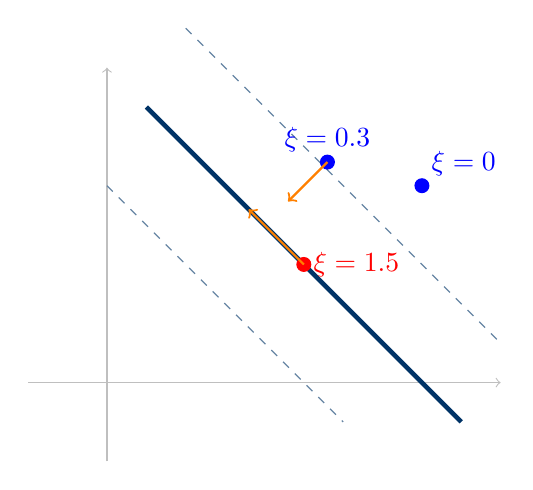
\begin{tikzpicture}[scale=1.0]
        \draw[->, gray!50] (-1,0) -- (5,0);
        \draw[->, gray!50] (0,-1) -- (0,4);
        \draw[ultra thick, DarkBlue] (0.5,3.5) -- (4.5,-0.5);
        \draw[dashed, DarkBlue!60] (0,2.5) -- (3,-0.5);
        \draw[dashed, DarkBlue!60] (1,4.5) -- (5,0.5);
        % Điểm
        \filldraw[blue] (4,2.5) circle (2.5pt) node[above right] {$\xi=0$};
        \filldraw[blue] (2.8,2.8) circle (2.5pt) node[above] {$\xi=0.3$};
        \draw[->, orange, thick] (2.8,2.8) -- (2.3,2.3);
        \filldraw[red] (2.5,1.5) circle (2.5pt) node[right] {$\xi=1.5$};
        \draw[->, orange, thick] (2.5,1.5) -- (1.8,2.2);
      \end{tikzpicture}
    \end{column}
  \end{columns}
\end{frame}

\begin{frame}{Tại sao ràng buộc lại là $y_i(\bm{w}^T\bm{x}_i + b) \ge 1 - \xi_i$?}
  \begin{block}{Gốc rễ: Yêu cầu về khoảng cách trong hard-margin}
    Trong không gian, khoảng cách từ điểm $\bm{x}_i$ đến siêu phẳng là $$\frac{|\bm{w}^T\bm{x}_i + b|}{\|\bm{w}\|}$$. \\
    Để đảm bảo độ rộng \textbf{margin} là $\frac{2}{\|\bm{w}\|}$, mọi điểm phải cách siêu phẳng \textbf{tối thiểu} $\frac{1}{\|\bm{w}\|}$. 
    
    \begin{center}
      Điều kiện đó được viết gọn thành: $y_i(\bm{w}^T\bm{x}_i + b) \ge 1$.
    \end{center}
  \end{block}

\end{frame}

\begin{frame}{Tại sao ràng buộc lại là $y_i(\bm{w}^T\bm{x}_i + b) \ge 1 - \xi_i$?}
    \textbf{Vậy $1 - \xi_i$ là gì?}
    \begin{itemize}
        \item $\xi_i$ là \textbf{khoảng cách vi phạm đã chuẩn hóa} (nhân với $\|\bm{w}\|$).
        \item Khi điểm $\bm{x}_i$ nằm quá gần hoặc sai phía, $y_i(\bm{w}^T\bm{x}_i + b)$ sẽ nhỏ hơn 1.
        \item Lượng thiếu hụt đó chính là $\xi_i$: 
        \[
        \xi_i = \max(0,\, 1 - y_i(\bm{w}^T\bm{x}_i + b))
        \]
        \item Do đó, yêu cầu $y_i(\bm{w}^T\bm{x}_i + b) \ge 1$ trở thành $y_i(\bm{w}^T\bm{x}_i + b) \ge 1 - \xi_i$.
    \end{itemize}
    \begin{exampleblock}{Ví dụ trực quan}
    \begin{itemize}
      \item Điểm A có $y_i(\bm{w}^T\bm{x}_i + b) = 0.7$. $\Rightarrow \xi_i = 1 - 0.7 = 0.3$ (Điểm lấn vào Margin).
      \item Điểm B có $y_i(\bm{w}^T\bm{x}_i + b) = -0.5$. $\Rightarrow \xi_i = 1 - (-0.5) = 1.5$ (Điểm bị phân loại Sai).
    \end{itemize}
    \textit{$\Rightarrow$ $\xi_i$ chính là câu trả lời cho câu hỏi: "Điểm này còn cách yêu cầu tối thiểu bao xa?"}
  \end{exampleblock}
\end{frame}

% ======================================================
% Thiết lập mô hình Soft-margin 
% ======================================================
\begin{frame}{Thiết lập bài toán soft-margin SVM}
  Để mô hình hóa bài toán với dữ liệu nhiễu, ta kết hợp hai thành phần:
  
  \begin{itemize}
    \item \textbf{Thành phần hình học ($\mathbf{w}, b$):} 
    Xác định siêu phẳng phân hoạch và độ rộng lề (Margin). Mục tiêu cốt lõi là tối đa hóa lề hình học $M = \frac{2}{\|\mathbf{w}\|}$.
    
    \item \textbf{Biến bù (slack variable $\xi_i$):} 
    Đóng vai trò là \textit{\textbf{sai số cho phép}} cho mỗi điểm dữ liệu $\mathbf{x}_i$:
    \begin{itemize}
      \item $\xi_i = 0$: Điểm nằm đúng phía và ngoài \textit{margin}.
      \item $0 < \xi_i \le 1$: Điểm nằm trong vùng \textit{margin} nhưng vẫn đúng phía.
      \item $\xi_i > 1$: Điểm bị phân loại sai (nằm sai phía siêu phẳng).
    \end{itemize}
  \end{itemize}
  
  \vspace{0.3cm}
  \textbf{Tư duy tối ưu:} Tìm sự cân bằng giữa việc \textit{giữ lề rộng nhất có thể} và \textit{giảm thiểu tổng mức độ vi phạm}.
\end{frame}

\begin{frame}{Soft-Margin SVM: Hàm mục tiêu và Ràng buộc}
  \begin{exampleblock}{Hàm mục tiêu}
    \[
    \min_{\mathbf{w}, b, \bm{\xi}} \quad \frac{1}{2}\|\mathbf{w}\|^2 + C \sum_{i=1}^n \xi_i
    \]
    \vspace{-0.3cm}
    \begin{itemize}
      \item $\frac{1}{2}\|\mathbf{w}\|^2$: margin rộng $\Leftrightarrow$ tổng quát hóa tốt.
      \item $\sum \xi_i$: tổng mức vi phạm margin (sai số).
    \end{itemize}
  \end{exampleblock}

  \begin{block}{Ràng buộc}
    \[
    y_i(\mathbf{w}^T \mathbf{x}_i + b) \ge 1 - \xi_i, \quad \xi_i \ge 0
    \]
  \end{block}

  \begin{alertblock}{Hinge Loss}
    $$\xi_i = \max(0,\, 1 - y_i(\mathbf{w}^T \mathbf{x}_i + b))$$
  \end{alertblock}

  \textbf{Tham số $C$:} Lớn $\rightarrow$ ít sai, margin hẹp; Nhỏ $\rightarrow$ margin rộng, chấp nhận nhiễu.
\end{frame}
\section{Kernel Trick}

\begin{frame}{Hạn chế của SVM tuyến tính}
  \begin{itemize}
    \item Cả Hard-Margin và Soft-Margin đều tìm \textbf{siêu phẳng tuyến tính}.
    \item Thực tế: nhiều tập dữ liệu có \textbf{ranh giới phi tuyến} (đường cong, vòng tròn).
    \item SVM tuyến tính thất bại hoàn toàn – dù có thêm slack $\xi_i$ cũng không giải quyết được.
  \end{itemize}
  \vspace{0.3cm}
  \centering
  \textbf{→ Cần một cách để mở rộng SVM sang các ranh giới phi tuyến.}
\end{frame}

\begin{frame}{Ví dụ: Dữ liệu hai vòng tròn đồng tâm}
  \begin{columns}
    \begin{column}{0.4\textwidth}
      \begin{itemize}
        \item Lớp trong (đỏ) và lớp ngoài (xanh)
        \item \textbf{Không} đường thẳng nào phân tách được hai lớp; Soft‑margin vẫn bất lực vì bản chất tuyến tính.
      \end{itemize}
    \end{column}
    \begin{column}{0.6\textwidth}
      \centering
      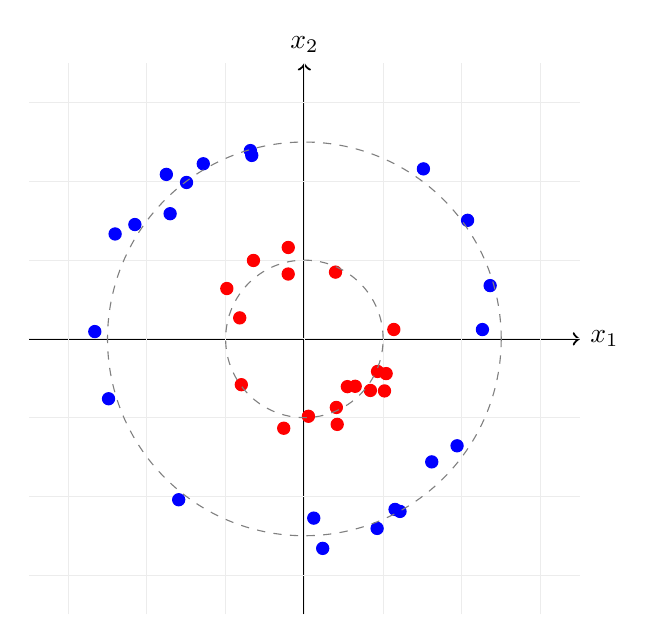
\begin{tikzpicture}[scale=1.0]
        % Trục tọa độ
        \draw[->, thick] (-3.5,0) -- (3.5,0) node[right] {$x_1$};
        \draw[->, thick] (0,-3.5) -- (0,3.5) node[above] {$x_2$};
        
        % Lưới mờ
        \draw[gray!15, thin] (-3.5,-3.5) grid (3.5,3.5);
        
        % Lớp ngoài (xanh) - bán kính ~2.5 ± nhiễu
        \foreach \i in {1,...,22} {
            \pgfmathsetmacro{\ang}{random(0,360)}
            \pgfmathsetmacro{\rad}{2.5 + 0.35*rand}
            \filldraw[blue] ({\rad*cos(\ang)}, {\rad*sin(\ang)}) circle (2.2pt);
        }
        
        % Lớp trong (đỏ) - bán kính ~1.0 ± nhiễu
        \foreach \i in {1,...,18} {
            \pgfmathsetmacro{\ang}{random(0,360)}
            \pgfmathsetmacro{\rad}{1.0 + 0.25*rand}
            \filldraw[red] ({\rad*cos(\ang)}, {\rad*sin(\ang)}) circle (2.2pt);
        }
        
        % Đường tròn tham khảo mờ
        \draw[gray, dashed, thin] (0,0) circle (1.0);
        \draw[gray, dashed, thin] (0,0) circle (2.5);
      \end{tikzpicture}
    \end{column}
  \end{columns}
\end{frame}

% ======================================
% Giới thiệu về phép phi tuyến
% ======================================

\begin{frame}{Ý tưởng: Ánh xạ đặc trưng $\phi(\mathbf{x})$}
  \begin{itemize}
    \item Ánh xạ dữ liệu từ không gian gốc $\mathbb{R}^d$ lên không gian $\mathbb{R}^D$ ($D > d$, thường $D \gg d$).
    \item Trong không gian mới, dữ liệu có thể trở nên \textbf{tuyến tính khả tách}.
  \end{itemize}
  \begin{exampleblock}{Ví dụ đơn giản}
    Với dữ liệu 2D: $X = (x_1, x_2) \in \mathbb{R}^2$, hai lớp đan xen. \\
    Ánh xạ $X' = \phi(X) = (x_1, x_2, x_1^2 + x_2^2)$ lên 3D $\rightarrow$ dùng siêu phẳng phân tách dễ dàng.
  \end{exampleblock}
  \begin{itemize}
    \item SVM trong không gian đặc trưng: thay $\mathbf{x}$ bằng $\phi(\mathbf{x})$.
  \end{itemize}
\end{frame}

\begin{frame}{Ví dụ: Ánh xạ hai vòng tròn đồng tâm}
  \begin{figure}
    \centering
    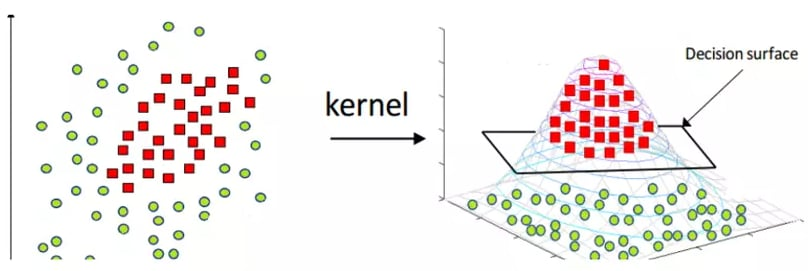
\includegraphics[width=0.7\textwidth, keepaspectratio]{img/chapter_03/kernel_trick_svm.jpg}
    \caption{Dữ liệu gốc 2D (trái) và sau khi ánh xạ lên 3D (phải)}
  \end{figure}

  
  \vspace{-0.3cm}
  \begin{columns}[T]
    \begin{column}{0.5\textwidth}
      \textbf{Không gian gốc 2D:}
      \begin{itemize}
        \item Hai lớp tạo thành vòng tròn đồng tâm.
        \item Không đường thẳng nào phân tách được.
        \item Cần ánh xạ lên không gian cao hơn.
      \end{itemize}
    \end{column}
    \begin{column}{0.5\textwidth}
      \textbf{Sau khi thêm đặc trưng $z = x_1^2 + x_2^2$:}
      \begin{itemize}
        \item Dữ liệu trải ra theo trục $z$ (bán kính).
        \item Lớp trong có $z \approx 1$, lớp ngoài $z \approx 4$.
        \item Có thể dùng một siêu phẳng (ở đây là mặt phẳng) phân tách dễ dàng.
      \end{itemize}
    \end{column}
  \end{columns}
  

\end{frame}



% ============================================
% Kernel Trick
% =============================================
\begin{frame}{Tổng quát hóa ánh xạ đặc trưng $\phi(\mathbf{x})$}
  \begin{alertblock}{Tại sao cần nhiều đặc trưng phi tuyến?}
    Trong thực tế, ta không biết trước đặc trưng nào giúp tuyến tính hóa dữ liệu. Do đó, ta thường bổ sung một tập lớn các đặc trưng:
    \[
    \phi(\mathbf{x}) = (1,\; x_1,\; x_2,\; x_1^2,\; x_2^2,\; x_1 x_2,\; \dots)
    \]
  \end{alertblock}
  
  \begin{itemize}
    \item Với $\phi(\mathbf{x})$, ta hy vọng tìm được siêu phẳng trong không gian mới phân tách tốt dữ liệu.
    \item \textbf{Nhưng:} số chiều $D$ của $\phi(\mathbf{x})$ có thể rất lớn (thậm chí vô hạn).
  \end{itemize}
\end{frame}

\begin{frame}{Thách thức của SVMs trong không gian đặc trưng}
  \begin{block}{Bài toán gốc với $\phi(\mathbf{x})$}
    \[
    \min_{\mathbf{w}, b} \frac{1}{2}\|\mathbf{w}\|^2 \quad \text{s.t.} \quad y_i(\mathbf{w}^T \phi(\mathbf{x}_i) + b) \ge 1
    \]
  \end{block}
  
  \begin{itemize}
    \item $\mathbf{w}$ có số chiều bằng với số chiều của $\phi(\mathbf{x})$, tức là $D$.
    \item Nếu $D$ rất lớn, việc lưu trữ và tính toán với $\mathbf{w}$ trở nên \textbf{bất khả thi}.
    \item Tính $\phi(\mathbf{x}_i)$ cho mọi điểm cũng cực kỳ tốn kém.
  \end{itemize}
  
  \begin{exampleblock}{Cần một cách tiếp cận khác}
    Làm sao để giải SVM mà không cần làm việc trực tiếp với vector $\mathbf{w}$ khổng lồ?
  \end{exampleblock}
\end{frame}


\begin{frame}{Bài toán đối ngẫu}
  \begin{block}{Bài toán đối ngẫu (Dual Form)}
    Khi chuyển sang bài toán đối ngẫu, vector $\mathbf{w}$ bị triệt tiêu. Hàm mục tiêu mới \textbf{chỉ phụ thuộc vào tích vô hướng} giữa các điểm trong không gian đặc trưng:
    \[
    \phi(\mathbf{x}_i)^T \phi(\mathbf{x}_j)
    \]
  \end{block}
  
  \begin{itemize}
    \item Vector trọng số được biểu diễn qua dữ liệu: $\mathbf{w} = \sum_{i} \alpha_i y_i \phi(\mathbf{x}_i)$.
    \item Hàm quyết định cũng chỉ cần tích vô hướng: $f(\mathbf{x}) = \sum_{i} \alpha_i y_i \phi(\mathbf{x}_i)^T \phi(\mathbf{x}) + b$.
  \end{itemize}
  
  \begin{alertblock}{Hệ quả then chốt}
    Nếu có cách tính $\phi(\mathbf{x}_i)^T \phi(\mathbf{x}_j)$ \textbf{trực tiếp} từ $\mathbf{x}_i, \mathbf{x}_j$ mà không cần biết $\phi$, ta sẽ giải quyết được bài toán trong không gian cao chiều một cách hiệu quả.
  \end{alertblock}
\end{frame}

% PHỤ LỤC 1 - CHỨNG MINH ĐỐI NGẪU
% \begin{frame}{Tại sao bài toán đối ngẫu chỉ cần $\phi(\mathbf{x}_i)^T \phi(\mathbf{x}_j)$?}
%   \begin{block}{Bài toán gốc trong không gian đặc trưng}
%     \[
%     \min_{\mathbf{w}, b} \frac{1}{2}\|\mathbf{w}\|^2 \quad \text{s.t.} \quad y_i(\mathbf{w}^T \phi(\mathbf{x}_i) + b) \ge 1, \forall i
%     \]
%   \end{block}

%   \begin{itemize}
%     \item Dùng phương pháp nhân tử Lagrange, ta thu được \textbf{bài toán đối ngẫu}:
%   \end{itemize}

%   \begin{exampleblock}{Hàm đối ngẫu (Dual Objective)}
%     \[
%     \max_{\bm{\alpha}} \sum_{i=1}^n \alpha_i - \frac{1}{2} \sum_{i=1}^n \sum_{j=1}^n \alpha_i \alpha_j y_i y_j \textcolor{DarkBlue}{\phi(\mathbf{x}_i)^T \phi(\mathbf{x}_j)}
%     \]
%     với $\alpha_i \ge 0$ và $\sum \alpha_i y_i = 0$.
%   \end{exampleblock}
% \end{frame}

% \begin{frame}{Tại sao bài toán đối ngẫu chỉ cần $\phi(\mathbf{x}_i)^T \phi(\mathbf{x}_j)$?}
%   \begin{exampleblock}{Hàm đối ngẫu (Dual Objective)}
%     \[
%     \max_{\bm{\alpha}} \sum_{i=1}^n \alpha_i - \frac{1}{2} \sum_{i=1}^n \sum_{j=1}^n \alpha_i \alpha_j y_i y_j \textcolor{DarkBlue}{\phi(\mathbf{x}_i)^T \phi(\mathbf{x}_j)}
%     \]
%     với $\alpha_i \ge 0$ và $\sum \alpha_i y_i = 0$.
%   \end{exampleblock}

%   \begin{itemize}
%     \item \textbf{Nhận xét:} Vector $\mathbf{w}$ đã bị triệt tiêu. Toàn bộ bài toán chỉ còn phụ thuộc vào \textbf{tích vô hướng} $\phi(\mathbf{x}_i)^T \phi(\mathbf{x}_j)$.
%     \item Hàm quyết định cũng chỉ cần tích vô hướng:
%     \[
%     f(\mathbf{x}) = \sum_{i=1}^n \alpha_i y_i \textcolor{DarkBlue}{\phi(\mathbf{x}_i)^T \phi(\mathbf{x})} + b
%     \]
%   \end{itemize}

%   \begin{alertblock}{Hệ quả quan trọng}
%     Nếu có cách tính $\phi(\mathbf{x}_i)^T \phi(\mathbf{x}_j)$ \textbf{trực tiếp} từ $\mathbf{x}_i, \mathbf{x}_j$ mà không cần biết $\phi$, ta sẽ tiết kiệm được chi phí tính toán khổng lồ.
%   \end{alertblock}
% \end{frame}


\begin{frame}{Vấn đề phát sinh với bài toán đối ngẫu}
    \begin{alertblock}{Vấn đề phát sinh}
        \begin{itemize}
        \item Khi số chiều $D$ của $\phi(\mathbf{x})$ rất lớn (thậm chí vô hạn), việc tính trực tiếp $\phi(\mathbf{x})$ (hay kể cả $\phi(\mathbf{x}_i)^T \phi(\mathbf{x}_j)$) trở nên \textbf{bất khả thi}.
        \item SVM cần tính rất nhiều tích vô hướng – nếu $D = 10^6$, mỗi phép nhân tốn $O(D)$.
        \end{itemize}
    \end{alertblock}

\end{frame}



\begin{frame}{Kernel Trick}
  \begin{block}{Ý tưởng cốt lõi}
    Thay vì tính $\phi(\mathbf{x})$ rồi lấy tích vô hướng, ta định nghĩa một hàm \textbf{kernel} $K(\mathbf{x}_i, \mathbf{x}_j)$ sao cho:
    \[
    K(\mathbf{x}_i, \mathbf{x}_j) = \phi(\mathbf{x}_i)^T \phi(\mathbf{x}_j)
    \]
    và tính \textbf{trực tiếp} từ $\mathbf{x}_i, \mathbf{x}_j$ trong không gian gốc.
  \end{block}

  \begin{exampleblock}{Ví dụ cụ thể với $\phi(\mathbf{x}) = (x_1^2, \sqrt{2}x_1 x_2, x_2^2)$}
    \begin{itemize}
      \item Tích vô hướng trong không gian đặc trưng: $\phi(\mathbf{x})^T \phi(\mathbf{z}) = x_1^2 z_1^2 + 2 x_1 x_2 z_1 z_2 + x_2^2 z_2^2 = (\mathbf{x}^T \mathbf{z})^2$
      \item Vậy chỉ cần dùng \textbf{kernel đa thức bậc 2}: $K(\mathbf{x}, \mathbf{z}) = (\mathbf{x}^T \mathbf{z})^2$.
    \end{itemize}
  \end{exampleblock}

  \begin{itemize}
    \item Chi phí tính toán: $O(d)$ trong không gian gốc thay vì $O(D)$ với $D \gg d$ (thậm chí $D = \infty$).
    \item Kernel phải thỏa mãn \textbf{điều kiện Mercer} (đảm bảo tồn tại không gian đặc trưng tương ứng).
  \end{itemize}
\end{frame}

\begin{frame}{Một số kernel phổ biến}
  \begin{columns}[T]
    \begin{column}{0.5\textwidth}
      \textbf{Linear Kernel}
      \[
      K(\mathbf{x}_i, \mathbf{x}_j) = \mathbf{x}_i^T \mathbf{x}_j
      \]
      \begin{itemize}
        \item Tương đương SVM tuyến tính.
        \item Dùng khi dữ liệu gần tuyến tính.
      \end{itemize}
      \vspace{0.3cm}
      \textbf{Polynomial Kernel}
      \[
      K(\mathbf{x}_i, \mathbf{x}_j) = (\gamma \mathbf{x}_i^T \mathbf{x}_j + r)^d
      \]
      \begin{itemize}
        \item $d$: bậc đa thức.
        \item Phù hợp với ranh giới dạng đa thức.
      \end{itemize}
    \end{column}
    \begin{column}{0.5\textwidth}
      \textbf{RBF (Gaussian) Kernel}
      \[
      K(\mathbf{x}_i, \mathbf{x}_j) = \exp\left(-\gamma \|\mathbf{x}_i - \mathbf{x}_j\|^2\right)
      \]
      \begin{itemize}
        \item Kernel được dùng \textbf{nhiều nhất}.
        \item Tương ứng không gian đặc trưng vô hạn chiều.
        \item $\gamma > 0$: tham số điều chỉnh độ phức tạp.
      \end{itemize}
    \end{column}
  \end{columns}
\end{frame}

\begin{frame}{Ảnh hưởng của $\gamma$ trong RBF Kernel}
  \begin{figure}
    \centering
    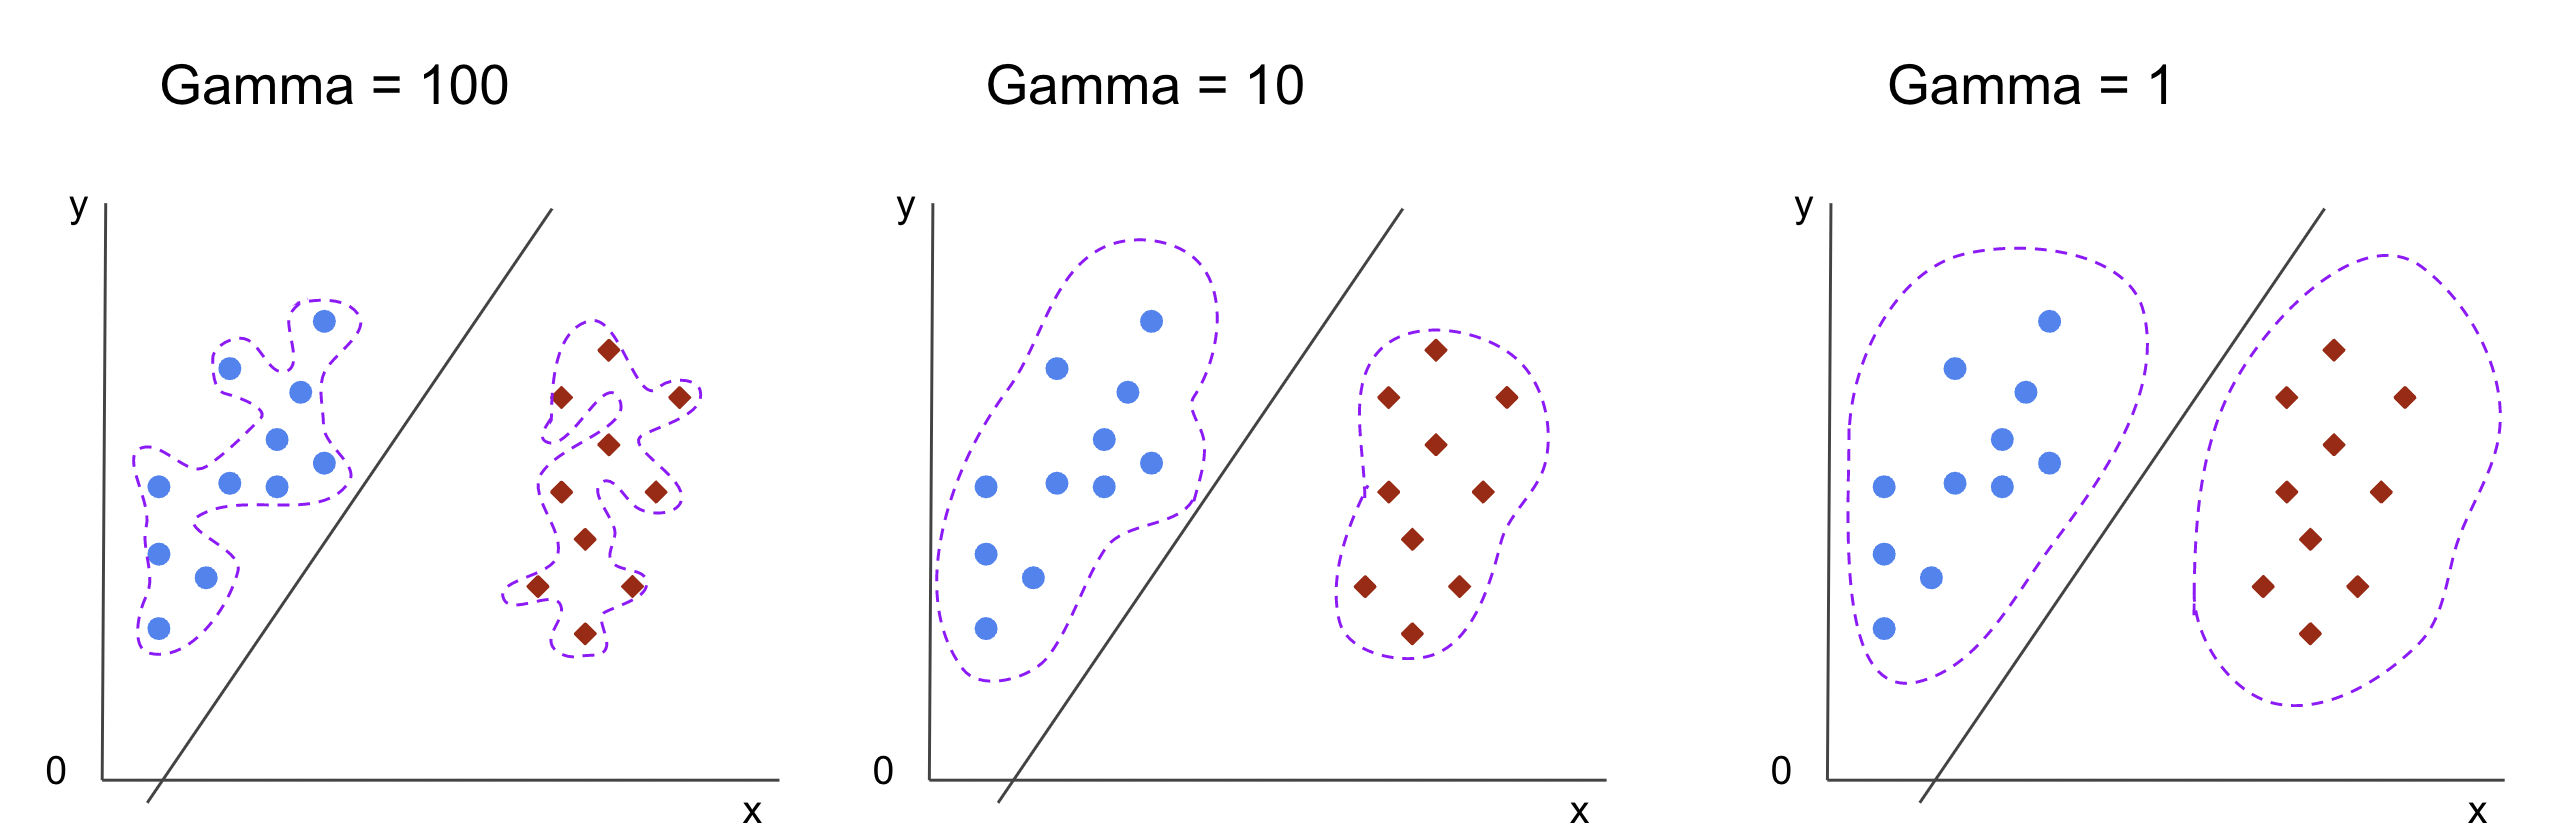
\includegraphics[width=0.8\textwidth, keepaspectratio]{img/chapter_03/gamma.png}
    \caption{Minh họa ranh giới phân loại với $\gamma$ lớn (trái) và $\gamma$ nhỏ (phải)}
  \end{figure}
  \vspace{-0.2cm}
  \begin{columns}[T]
    \begin{column}{0.5\textwidth}
      \begin{itemize}
        \item $\gamma$ \textbf{nhỏ}: mỗi điểm ảnh hưởng rộng, ranh giới mượt, tổng quát hóa tốt.
      \end{itemize}
    \end{column}
    \begin{column}{0.5\textwidth}
      \begin{itemize}
        \item $\gamma$ \textbf{lớn}: mỗi điểm ảnh hưởng hẹp, ranh giới uốn theo dữ liệu, dễ overfitting.
      \end{itemize}
    \end{column}
  \end{columns}
\end{frame}

\begin{frame}{Tối ưu siêu tham số cho SVM với kernel}
  \begin{itemize}
    \item SVM với kernel (đặc biệt là RBF) có hai siêu tham số quan trọng:
      \begin{enumerate}
        \item \textbf{$C$}: cân bằng giữa độ rộng margin và mức phạt sai số.
        \item \textbf{$\gamma$}: kiểm soát độ phức tạp của ranh giới (độ uốn).
      \end{enumerate}
    \item Chọn thủ công khó đạt hiệu quả tối ưu.
  \end{itemize}

  \begin{block}{Phương pháp phổ biến: Grid Search kết hợp Cross-Validation}
    \begin{itemize}
      \item Thử nhiều cặp $(C, \gamma)$ trên lưới giá trị (ví dụ: $C \in \{0.1, 1, 10, 100\}$, $\gamma \in \{0.001, 0.01, 0.1, 1\}$).
      \item Đánh giá bằng cross‑validation, chọn cặp cho điểm tốt nhất.
      \item Trong thư viện \texttt{scikit-learn}: \texttt{GridSearchCV(SVC(), param\_grid, cv=5)}.
    \end{itemize}
  \end{block}
\end{frame}


\begin{frame}{Tổng kết: Kernel Trick}
  \begin{block}{Vấn đề}
    \textbf{SVM tuyến tính} (cả hard và soft margin) thất bại với dữ liệu có ranh giới phi tuyến.
  \end{block}
  \begin{block}{Giải pháp}
    \begin{itemize}
      \item Ánh xạ dữ liệu lên không gian đặc trưng cao chiều $\phi(\mathbf{x})$ để dữ liệu trở nên tuyến tính khả tách.
      \item Nhờ \textbf{bài toán đối ngẫu}, mọi tính toán chỉ cần \textbf{tích vô hướng} $\phi(\mathbf{x}_i)^T \phi(\mathbf{x}_j)$.
    \end{itemize}
  \end{block}
  \begin{exampleblock}{Kernel Trick}
    Dùng \textbf{hàm kernel} $K(\mathbf{x}_i, \mathbf{x}_j)$ tính trực tiếp tích vô hướng mà không cần biết $\phi$, cho phép làm việc với không gian vô hạn chiều (RBF) với chi phí tính toán thấp.
  \end{exampleblock}
  \begin{itemize}
    \item Hai siêu tham số chính với RBF kernel: $C$ (margin vs. sai số) và $\gamma$ (độ uốn ranh giới).
    \item Thực tế: tối ưu $(C,\gamma)$ bằng \textbf{grid-search} với \textbf{cross‑validation}.
  \end{itemize}
  \vspace{0.2cm}
  \centering
\end{frame}

\section{Kỹ thuật triển khai SVM}

\begin{frame}{Quy trình huấn luyện SVM điển hình}
  \begin{enumerate}
    \item \textbf{Thu thập và làm sạch dữ liệu}.
    \item \textbf{Tiền xử lý:}
      \begin{itemize}
        \item Chuẩn hóa đặc trưng (StandardScaler).
        \item Xử lý giá trị thiếu, mã hóa biến phân loại.
      \end{itemize}
    \item \textbf{Chọn kernel và mô hình:}
      \begin{itemize}
        \item Tuyến tính: \texttt{LinearSVC}.
        \item Phi tuyến: \texttt{SVC(kernel='rbf')}.
      \end{itemize}
    \item \textbf{Tối ưu siêu tham số} ($C$, $\gamma$) với Grid Search + Cross‑Validation.
    \item \textbf{Huấn luyện và đánh giá} trên tập test.
    \item \textbf{Triển khai} (lưu mô hình với \texttt{joblib} hoặc \texttt{pickle}).
  \end{enumerate}
\end{frame}

% ============================
% Tiền xử lý
% ===========================

\begin{frame}{Xử lý dữ liệu mất cân bằng}
  \begin{itemize}
    \item SVM cố gắng tối đa margin chung, có thể bỏ qua lớp thiểu số nếu không điều chỉnh.
    \item Giải pháp đơn giản trong sklearn: \texttt{class\_weight='balanced'}.
      \begin{itemize}
        \item Tự động tăng trọng số phạt $C$ cho các lớp ít mẫu.
      \end{itemize}
    \item Cũng có thể truyền dictionary trọng số tùy chỉnh: \texttt{class\_weight=\{0:1, 1:10\}}.
  \end{itemize}
  \begin{exampleblock}{Khi nào cần?}
    \begin{itemize}
      \item Tỉ lệ lớp chênh lệch lớn (ví dụ 1:10, 1:100).
      \item Bài toán cần recall cao cho lớp thiểu số (phát hiện gian lận, bệnh hiếm).
    \end{itemize}
  \end{exampleblock}
\end{frame}

\begin{frame}{Feature Scaling quan trọng như thế nào?}
  \begin{alertblock}{Tại sao SVM nhạy cảm với thang đo?}
    \begin{itemize}
      \item SVM dựa trên khoảng cách (margin) và tích vô hướng.
      \item Nếu một đặc trưng có giá trị lớn hơn hẳn, nó sẽ chi phối hàm mục tiêu và làm méo margin.
    \end{itemize}
  \end{alertblock}
  \begin{exampleblock}{Cách làm trong sklearn}
    \begin{itemize}
      \item Dùng \texttt{StandardScaler} để đưa mỗi đặc trưng về trung bình 0, độ lệch chuẩn 1.
      \item \textbf{Luôn} fit scaler trên tập huấn luyện, sau đó transform cho cả tập kiểm tra.
    \end{itemize}
  \end{exampleblock}
\end{frame}

\begin{frame}{Feature Scaling quan trọng như thế nào?}
  \begin{center}
    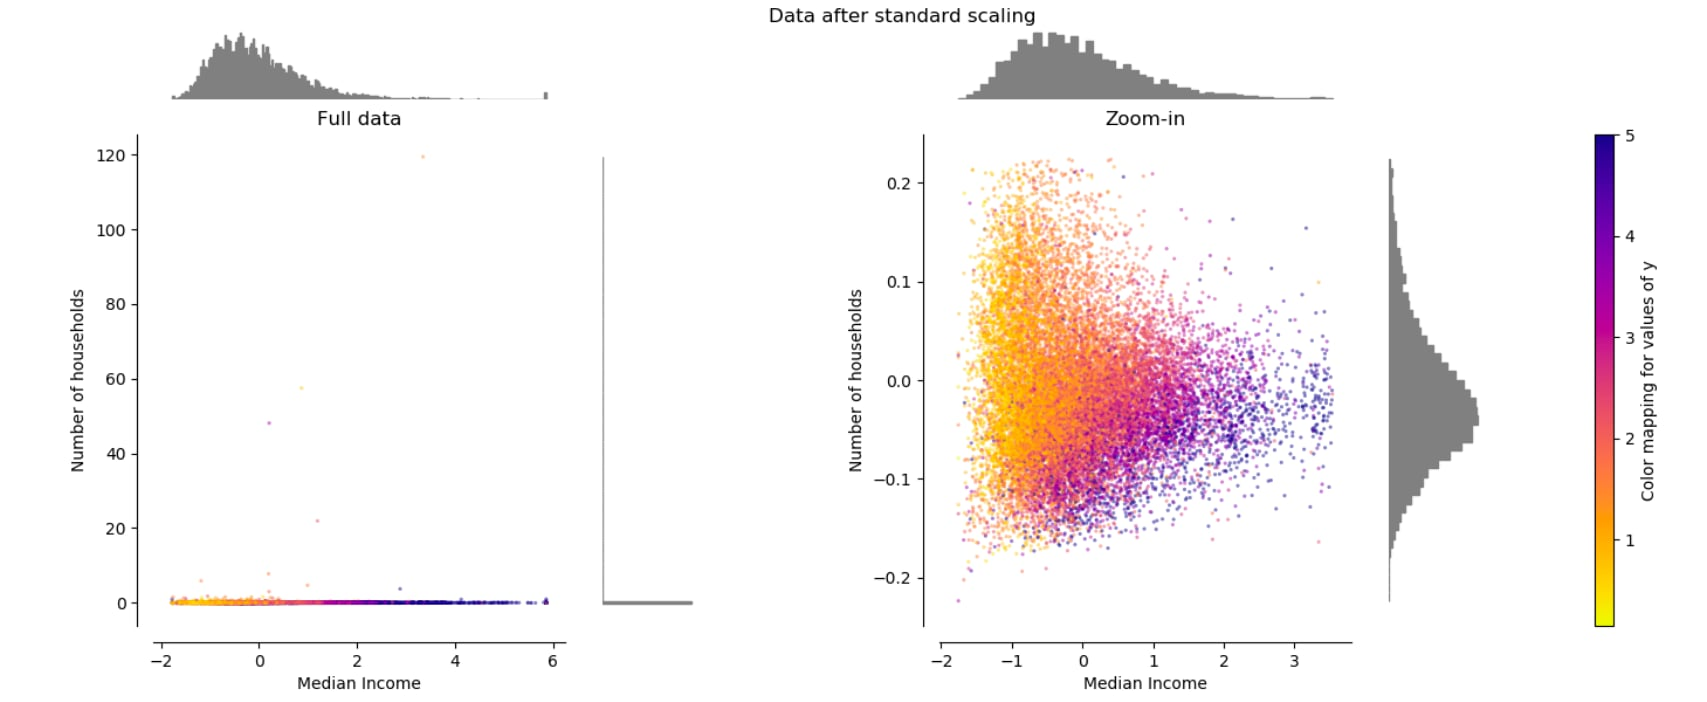
\includegraphics[width=\textwidth]{img/chapter_04/feature_scaling.jpg}
  \end{center}
\end{frame}

% ================================
% Triển khai SVM 
% ================================
\begin{frame}{LinearSVC vs SVC}
  \begin{columns}[T]
    \begin{column}{0.5\textwidth}
      \textbf{LinearSVC}
      \begin{itemize}
        \item Chuyên cho kernel tuyến tính.
        \item Tối ưu bằng thuật toán coordinate descent (nhanh, ít tốn RAM).
        \item Hỗ trợ dữ liệu thưa (sparse).
        \item \textbf{Dùng cho dữ liệu lớn} ($>10^5$ mẫu).
      \end{itemize}
    \end{column}
    \begin{column}{0.5\textwidth}
      \textbf{SVC(kernel='rbf')}
      \begin{itemize}
        \item Linh hoạt, xử lý ranh giới phi tuyến.
        \item Độ phức tạp $O(n^2)$ đến $O(n^3)$ về bộ nhớ/thời gian.
        \item Không phù hợp nếu $n > 10^4$–$10^5$.
        \item Có thể dùng \texttt{RBFSampler} để xấp xỉ kernel.
      \end{itemize}
    \end{column}
  \end{columns}
  \vspace{0.3cm}
  \begin{block}{Kinh nghiệm}
    \begin{itemize}
      \item Bắt đầu với LinearSVC (baseline). Nếu underfit, thử RBF.
      \item Với RBF, giảm số mẫu hoặc dùng xấp xỉ nếu dữ liệu quá lớn.
    \end{itemize}
  \end{block}
\end{frame}


\begin{frame}{Tối ưu $C$ và $\gamma$ với \texttt{GridSearchCV}}
  \begin{block}{Code mẫu}
    \begin{semiverbatim}
from sklearn.model\_selection import GridSearchCV

from sklearn.svm import SVC

param\_grid = \{

    'C': [0.1, 1, 10, 100],

    'gamma': [0.001, 0.01, 0.1, 1]

\}

grid = GridSearchCV(SVC(kernel='rbf'), param\_grid, cv=5)

grid.fit(X\_train\_scaled, y\_train)

print(grid.best\_params\_)
    \end{semiverbatim}
  \end{block}
  \begin{itemize}
    \item Luôn thực hiện cross‑validation (ví dụ cv=5) để đánh giá khách quan.
    \item Có thể dùng \texttt{RandomizedSearchCV} nếu không gian tham số quá lớn.
    \item Thời gian tìm kiếm tăng nhanh với số lượng mẫu – cân nhắc giảm lưới hoặc dùng tập con.
  \end{itemize}
\end{frame}


% ================================
% CÁC KHÍA CẠNH KHÁC
%================================
\begin{frame}{Lấy xác suất dự đoán từ SVM}
  \begin{itemize}
    \item Mặc định SVM chỉ trả về nhãn cứng ($\pm 1$) hoặc khoảng cách đến siêu phẳng.
    \item Để có xác suất (probability), cần bật \texttt{probability=True} khi khởi tạo SVC.
    \item Cơ chế: Platt scaling – hồi quy logistic trên output của SVM (tốn thêm thời gian huấn luyện).
  \end{itemize}
  \begin{block}{Lưu ý}
    \begin{itemize}
      \item Xác suất thu được có thể không được hiệu chuẩn tốt (calibrated) – cân nhắc dùng \texttt{CalibratedClassifierCV}.
      \item Không nên dùng probability nếu chỉ cần nhãn, vì làm chậm đáng kể.
    \end{itemize}
  \end{block}
\end{frame}

\begin{frame}{SVM với bài toán nhiều lớp (Multiclass)}
  \begin{itemize}
    \item SVM nguyên bản chỉ phân loại nhị phân.
    \item Để xử lý $K$ lớp ($K>2$), có hai chiến lược chính:
      \begin{enumerate}
        \item \textbf{One‑vs‑Rest (OvR)}: huấn luyện $K$ bộ SVM, mỗi bộ phân biệt một lớp với phần còn lại.
        \item \textbf{One‑vs‑One (OvO)}: huấn luyện $\binom{K}{2}$ bộ SVM, mỗi cặp lớp một bộ.
      \end{enumerate}
  \end{itemize}
  \begin{block}{Trong sklearn}
    \begin{itemize}
      \item \texttt{SVC} mặc định dùng \textbf{OvO} (phù hợp khi số lớp ít).
      \item \texttt{LinearSVC} mặc định dùng \textbf{OvR} (nhanh hơn cho nhiều lớp).
    \end{itemize}
  \end{block}
\end{frame}
\section{Practice: Phân loại ảnh số viết tay 0 và 1}

% ======================================
% Slide 5.1: Giới thiệu bài toán
% ======================================
\begin{frame}{Bài toán: Phân biệt chữ số 0 và 1}
  \begin{itemize}
    \item \textbf{Mục tiêu:} Xây dựng mô hình SVM phân loại ảnh chứa chữ số viết tay \textbf{0} và \textbf{1}.
    \item \textbf{Dữ liệu:} Sử dụng tập MNIST (hoặc phiên bản thu gọn) – ảnh xám kích thước $28 \times 28$ pixels.
    \item \textbf{Vì sao chọn SVM?}
      \begin{itemize}
        \item Dữ liệu nhỏ, số chiều trung bình ($784$).
        \item Ranh giới giữa 0 và 1 gần như tuyến tính khả tách.
        \item SVM hoạt động rất tốt trên bài toán này.
      \end{itemize}
  \end{itemize}
  \centering
  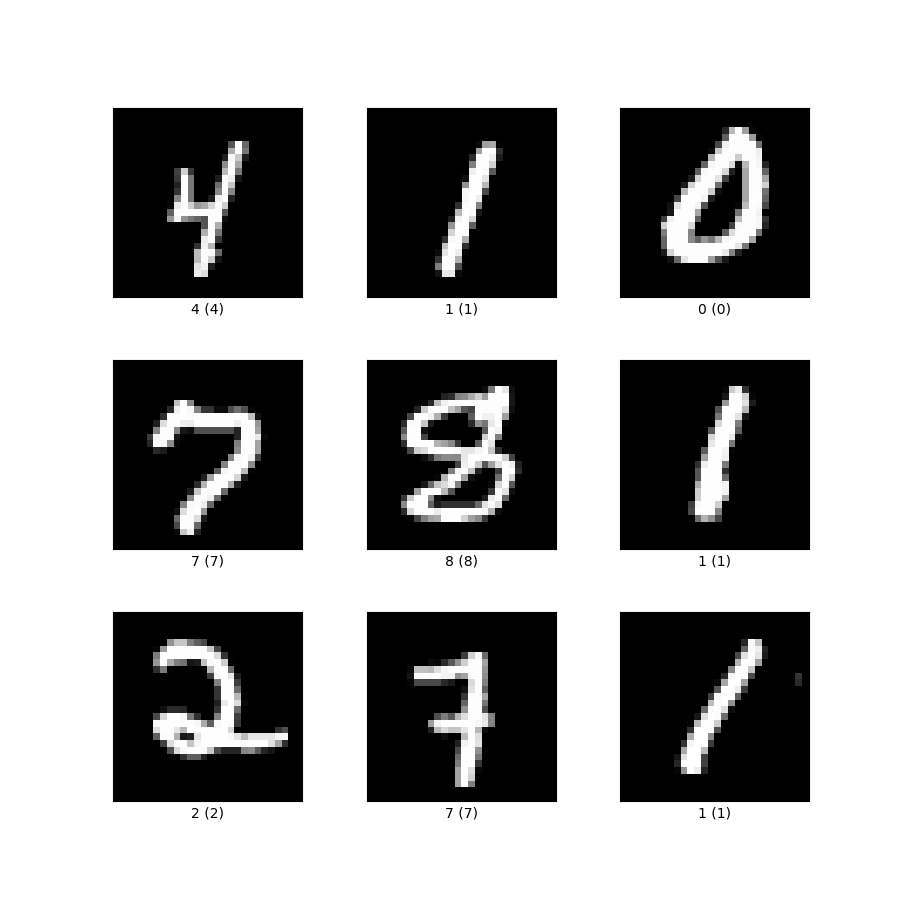
\includegraphics[width=0.25\textwidth]{img/chapter_05/mnist_samples.png}
\end{frame}

% ======================================
% Slide 5.2: Khám phá dữ liệu và tiền xử lý
% ======================================
\begin{frame}[fragile]{Tải dữ liệu và tiền xử lý}
  \begin{block}{Code tải và lọc dữ liệu}
    \begin{semiverbatim}
from sklearn.datasets import fetch_openml
from sklearn.model_selection import train_test_split

mnist = fetch_openml('mnist_784', version=1)
X, y = mnist.data, mnist.target.astype(int)
mask = (y == 0) | (y == 1)
X_bin, y_bin = X[mask], y[mask]
    \end{semiverbatim}
  \end{block}
  \begin{itemize}
    \item \textbf{Phẳng hóa:} Ảnh $28 \times 28$ được duỗi thành vector $784$ chiều.
    \item \textbf{Chuẩn hóa:} Dùng \texttt{StandardScaler} để đưa dữ liệu về phân phối chuẩn.
  \end{itemize}
  \begin{exampleblock}{Lưu ý}
    Với SVM, \textbf{luôn chuẩn hóa} dữ liệu trước khi huấn luyện!
  \end{exampleblock}
\end{frame}

\begin{frame}{EDA: Phân phối nhãn và ảnh trung bình}
  \begin{columns}[T]
    \begin{column}{0.5\textwidth}
      \centering
      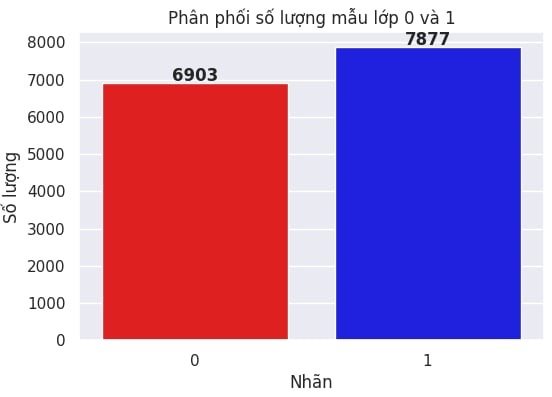
\includegraphics[width=0.7\textwidth, keepaspectratio]{img/chapter_05/label_distribution.jpg}
      \begin{itemize}
        \item Dữ liệu khá cân bằng giữa hai lớp 0 và 1.
        \item Không cần áp dụng kỹ thuật cân bằng lớp.
      \end{itemize}
    \end{column}
    \begin{column}{0.5\textwidth}
      \centering
      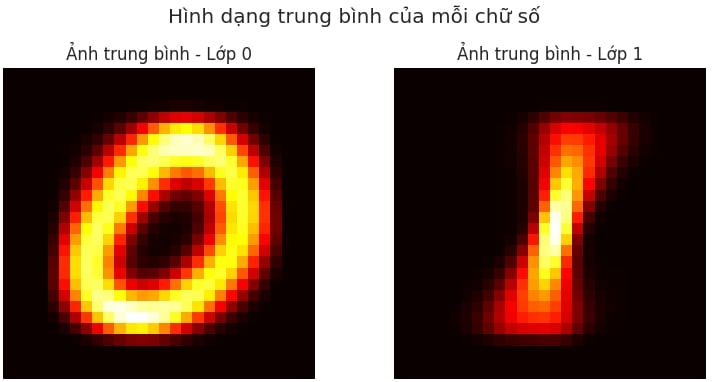
\includegraphics[width=0.7\textwidth, keepaspectratio]{img/chapter_05/average_image.jpg}
      \begin{itemize}
        \item Ảnh trung bình cho thấy sự khác biệt rõ rệt về hình dạng.
        \item Lớp 0 có xu hướng tròn, lớp 1 có nét thẳng đứng.
      \end{itemize}
    \end{column}
  \end{columns}
  \vspace{0.2cm}
  \begin{block}{Nhận xét}
    Hai lớp có đặc trưng trực quan khá khác biệt, gợi ý rằng một mô hình tuyến tính có thể phân tách tốt.
  \end{block}
\end{frame}

\begin{frame}{EDA: Phân bố cường độ pixel}
  \centering
  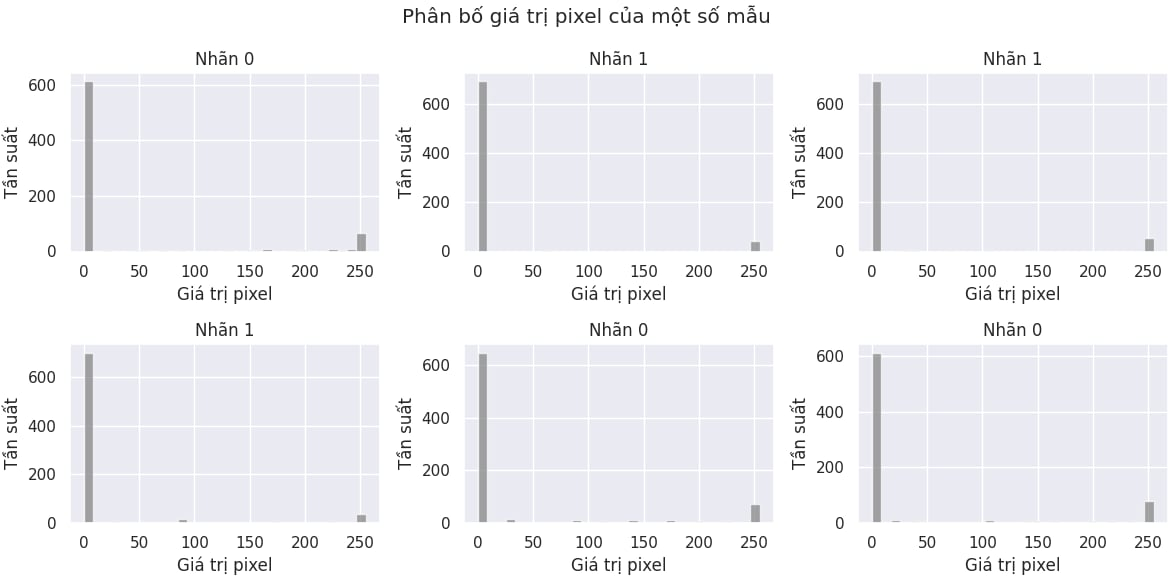
\includegraphics[width=0.7\textwidth, keepaspectratio]{img/chapter_05/pixel_i_distribution.jpg}
  \vspace{0.2cm}
  \begin{itemize}
    \item Biểu đồ histogram cho thấy phần lớn pixel có giá trị thấp (nền tối).
    \item Các pixel sáng tập trung ở vùng chữ viết, tạo nên đặc trưng phân biệt.
    \item \textbf{Chuẩn hóa dữ liệu} (StandardScaler) là cần thiết để SVM không bị ảnh hưởng bởi thang đo.
  \end{itemize}
\end{frame}

% ======================================
% Slide 5.3: Xây dựng mô hình SVM tuyến tính
% ======================================
\begin{frame}[fragile]{Huấn luyện SVM tuyến tính (LinearSVC)}
  \begin{block}{Pipeline đầy đủ}
    \begin{semiverbatim}
from sklearn.pipeline import Pipeline
from sklearn.preprocessing import StandardScaler
from sklearn.svm import LinearSVC

pipeline = Pipeline([
    ('scaler', StandardScaler()),
    ('svm', LinearSVC(C=1.0, max_iter=10000))
])
pipeline.fit(X_train, y_train)
accuracy = pipeline.score(X_test, y_test)
print(f'Accuracy: {accuracy:.4f}')
    \end{semiverbatim}
  \end{block}

\end{frame}

\begin{frame}[fragile]{Huấn luyện SVM tuyến tính (LinearSVC)}
    \begin{itemize}
        \item \textbf{Tham số $C$:} Giữ mặc định $1.0$ (có thể tinh chỉnh sau).
        \item \textbf{max\_iter:} Tăng lên để đảm bảo hội tụ.
    \end{itemize}
\end{frame}
% ======================================
% Slide 5.4: Đánh giá mô hình chi tiết
% ======================================
\begin{frame}{Đánh giá mô hình}
  \begin{columns}
    \begin{column}{0.5\textwidth}
      \textbf{Confusion Matrix}
      \begin{itemize}
        \item True Positive (1 được đoán đúng)
        \item True Negative (0 được đoán đúng)
        \item False Positive / Negative
      \end{itemize}
      \vspace{0.2cm}
      \centering
      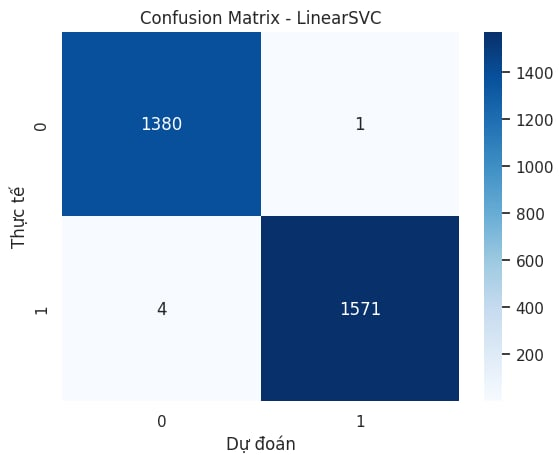
\includegraphics[width=0.8\textwidth]{img/chapter_05/confusion_matrix_linearSVM.jpg}
    \end{column}
    \begin{column}{0.5\textwidth}
      \textbf{Các metric}
      \begin{itemize}
        \item Accuracy: $\frac{TP+TN}{Total}$
        \item Precision: $\frac{TP}{TP+FP}$
        \item Recall: $\frac{TP}{TP+FN}$
        \item F1-score
      \end{itemize}
      \begin{exampleblock}{Kết quả điển hình}
        Với 0 vs 1, accuracy thường đạt \textbf{>99.5\%}.
      \end{exampleblock}
    \end{column}
  \end{columns}
\end{frame}

% ======================================
% Slide 5.5: Trực quan hóa Support Vectors
% ======================================
\begin{frame}{Trực quan hóa Support Vectors}
  \begin{itemize}
    \item Mỗi điểm dữ liệu có hệ số $\alpha_i$. Nếu $\alpha_i > 0$, điểm đó là \textbf{support vector}.
    \item Support vectors nằm trên hoặc trong lề margin, quyết định vị trí siêu phẳng.
    \item Đối với LinearSVC, có thể truy cập thuộc tính \texttt{svm.coef\_} và \texttt{svm.intercept\_}.
  \end{itemize}
  \vspace{0.2cm}
  \begin{block}{Minh họa (sau khi giảm chiều về 2D)}
    \centering
    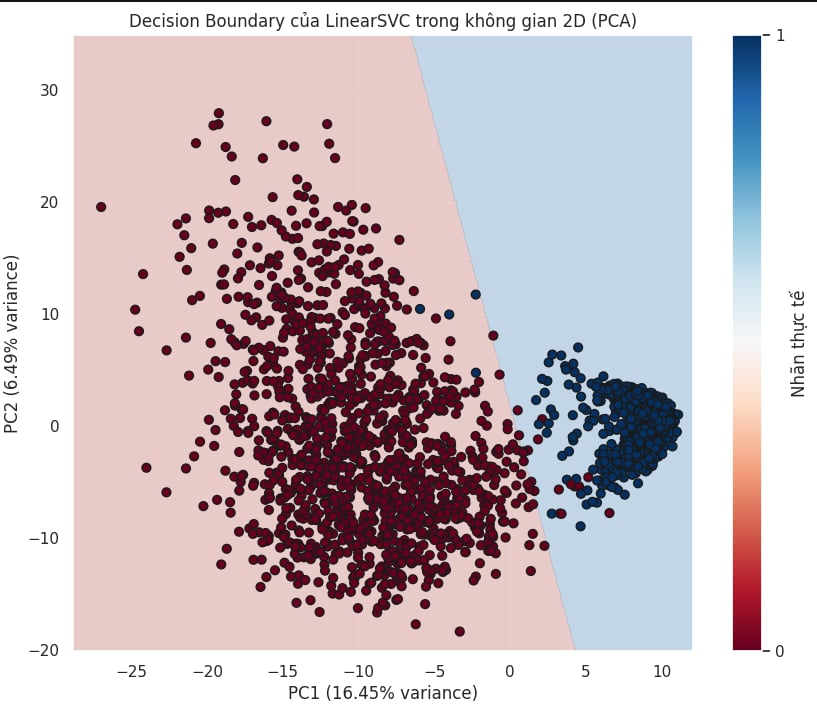
\includegraphics[width=0.45\textwidth]{img/chapter_05/decision_boundary.jpg}
  \end{block}
\end{frame}

% ======================================
% Slide 5.6: So sánh với Kernel RBF
% ======================================
\begin{frame}[fragile]{Thử nghiệm với Kernel RBF}
  \begin{block}{Code so sánh}
    \begin{semiverbatim}
from sklearn.svm import SVC

pipeline_rbf = Pipeline([
    ('scaler', StandardScaler()),
    ('svm', SVC(kernel='rbf', C=1.0, gamma='scale'))
])
pipeline_rbf.fit(X_train, y_train)
print(pipeline_rbf.score(X_test, y_test))
    \end{semiverbatim}
  \end{block}
  \begin{itemize}
    \item Với bài toán 0 vs 1, RBF không cải thiện đáng kể (vẫn ~99.5\%).
    \item \textbf{Thời gian huấn luyện} chậm hơn đáng kể so với LinearSVC.
    \item Kết luận: Chỉ dùng kernel phi tuyến khi thực sự cần thiết.
  \end{itemize}
\end{frame}

% ======================================
% Slide 5.7: Tổng kết và lưu ý thực tế
% ======================================
\begin{frame}{Tổng kết: SVM cho bài toán ảnh}
  \begin{itemize}
    \item \textbf{Quy trình chuẩn:}
      \begin{enumerate}
        \item Flatten ảnh $\rightarrow$ vector.
        \item Chuẩn hóa (StandardScaler).
        \item Chọn mô hình: LinearSVC cho nhanh, SVC+RBF nếu cần phi tuyến.
        \item Đánh giá và tinh chỉnh.
      \end{enumerate}
    \item \textbf{Khi nào dùng SVM cho ảnh?}
      \begin{itemize}
        \item Dữ liệu nhỏ ($n < 10^4$).
        \item Đặc trưng đã được trích xuất tốt (HOG, embeddings).
        \item Cần mô hình giải thích được (support vectors).
      \end{itemize}
    \item \textbf{Hạn chế:}
      \begin{itemize}
        \item Không tận dụng được cấu trúc không gian 2D của ảnh.
        \item Khó mở rộng với ảnh lớn, nhiều lớp.
      \end{itemize}
  \end{itemize}
  \centering
  \textbf{$\rightarrow$ Với ảnh phức tạp, Deep Learning (CNN) là lựa chọn tốt hơn.}
\end{frame}

% ======================================
% Slide kết thúc chương (có thể là Q&A)
% ======================================
\begin{frame}{Q\&A – Thực hành SVM}
  \centering
  \Large
 Arigathanksssss \\
  \vspace{0.5cm}
  \normalsize
\end{frame}
% Bạn sẽ tạo và import chapter_03.tex sau

\end{document}